\section{Introduction}
We were asked for the course Architecture and Performance of Computer to
implement a cache server. The project was divided in two parts and the 
goal was to compare different caching mechanism based on a trace
of 3,079,312 requests which were provided to us.

\section{Warm-up phase}

On this plot, you can see how the hit rate evolves over time (over the
number of requests done). As we can
see, after 10,000 requests, we reach a constant hit rate so we think it is
a reasonable choice for a warm-up size to have results that make sense. 

\begin{figure}[!ht]
	\centering
	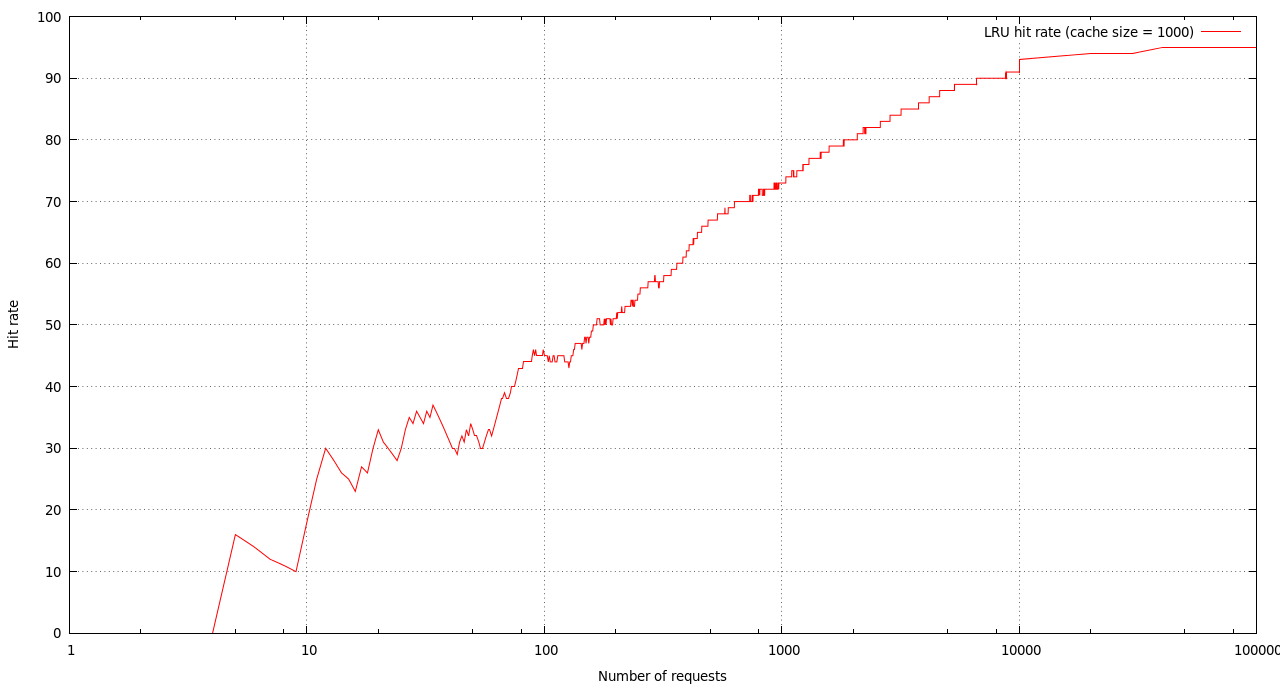
\includegraphics[width=\linewidth]{lru_hit_rate.png}
	\caption{Evaluation of a good warm up value}
\end{figure}
\FloatBarrier

\section{Task1.1}

\subsection{Results}
We can see on the Figure2 that LRU provide a better perfomance with the 
trace. We did not analyze the trace but an explanation might be the
problem of cache pollution.

\begin{figure}[!ht]
    \centering
    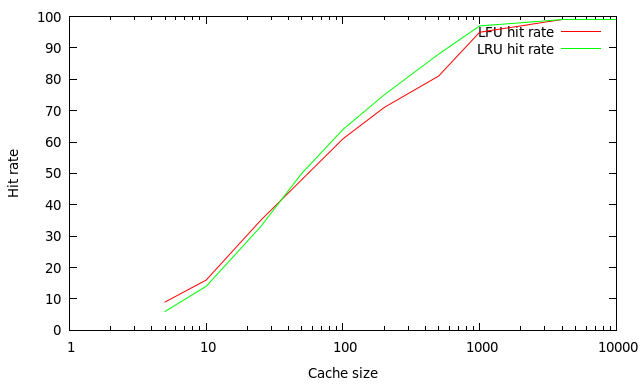
\includegraphics[width=\linewidth]{task1.png}
    \caption{LFU vs LRU implementation, 1 slot = 1 resource ; the y-axis is
    for the hit rate (in percentage), the x-axis is the number of slots
    (logarithmic). X = 10,000}
\end{figure}
\FloatBarrier

\subsection{LFU implementation description}
To implement the LFU we have decided to use an hashmap. The key used 
by the hashmap is the path to the requested object and the value is what
is requested (it's represented by the class RequestedObject). The removal
policy of the LFU is based on the access frequency of an object. To
implement this aspect, each object has an access counter which is 
incremented at each access. Because we used an hashmap, adding and
checking an element are done in O(1). The removal operation is less efficient,
because we have to iterate over the data structure to find the object with
the minimum access counter. \newline

If there are several object with the minimal access counter value, the first
one found will be removed. Because there no guarantee on the order of
the object in the hashmap (order of object does not depends on the 
insertion order). So it provides a random behaviour which is what we
were looking for as there is no defined strategies in this case and 
depending on the trace, some choice may be better than other one. 

\section{Task1.2}

\subsection{Results}

\begin{figure}[!ht]
    \centering
    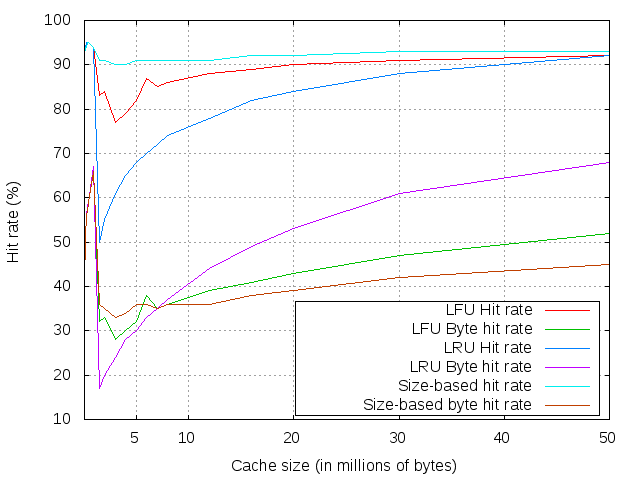
\includegraphics[width=\linewidth]{task2.png}
    \caption{Results of the task 2 (X = 10,000)}
\end{figure}
\FloatBarrier

\subsection{Chosen strategy}

We choose to implement the Remove Largest File strategy. It used an hashmap
to store the data, the keys are the name of the accessed resources and the
values are the related RequestedObject linked to the value. We also tested
the Remove Smallest File but the results in term of hit rates were worse,
it doesn't look like a good strategy to cache this trace.

\subsection{How the 3 strategies differ}

The Remove Largest File (RLF) strategy has the best hit rate, but the worst byte
hit rate. In this case, it is the strategy that gives the worst result. The
average strategy is the LFU strategy which gives decent results on our set
of data. The best strategy is clearly the LRU strategy which reaches 50\%
of byte hit rate with less than 20Mb of cache size. \newline

The reason for those results are that the trace is very big and contains a
lot of different data, The RLF strategy doesn't provide good results
because if you always remove the largest file, the miss (even if it happens
more rarely) are huge in terms of bytes. The LFU doesn't provide good
results because with some many data, we have cache pollution after a while.
The LRU results might be explained by the fact that the first accessed
resources are no more accessed after a while, replaced by new resources
which provides good result in this case. \newline
